\section{A new evaluation methodology}
\label{sec:methodology}

In \sectionref{analysis} we identified two main problems with the current evaluation methodology:
\begin{enumerate}
  \item A closed-window pooling evaluation is significantly biased
    against development systems, particularly those of new teams.
  \item Existing evaluation metrics have too much variance on the
    evaluation data to be a measure of performance that will generalize
    to new documents and queries.
\end{enumerate}

At the same time, we would like to capture some of the defining aspects of the original TAC-KBP evaluation:
\begin{enumerate}
  \item The evaluation should allow comparisons against human effort on the task. %TODO: reason?
  \item Scores should be aggregated over entities, because entity-level scores are a more natural measure of knowledge base quality.
  \item Teams should be required to submit justifications for relations they predict, because this makes it possible to interpret and verify system output.
\end{enumerate}

Our goal in this section is to propose a new methodology that maintains the above elements while addressing the mentioned problems head on 
  by indefinitely opening the pooling evaluation window by making the evaluation online
  and by combining evaluation data for each team in statistically optimal fashion.
Before we describe the overview of our proposed evaluation platform, we take a brief detour to answer an important question.

\paragraph{Would a larger human-annotated dataset suffice?}
A natural question to ask before embarking on the significant effort of an online evaluation is whether a large-enough dataset could be reliably collected by spending a little more money. 

An important part of the KBP evaluation is to test on an unseen document collection.

A number of datasets for relation extraction, even on the TAC-KBP task, have been collected in the past, for example in the work of \citet{angeli2014combining}.
This dataset is very small and does not have sufficient coverage, but is useful for training.
Unfortunately, these datasets have also been collected by pooling responses.

Another way of empirically answering this question is to see how many contexts need be evaluated to reduce pooling bias sufficiently. We can extrapolate this number by studying how the pooling bias varies by the number of systems.
Using the 2015 evaluation data, we find that we would need to pool the output of \todo{100} systems with \todo{$10^6$} lines of output evaluated.
With the `anydoc' heuristic, this number is far less, but the error introduced by the heuristic also increases.
%TODO: graph.

We can estimate the cost of annotating such a large corpus by calculating how many documents need be exhaustively annotated by humans-- it comes out to \todo{\$10 million}. 
We believe this is reasonable justification to discard the static dataset approach and embrace an online evaluation wherein systems are continuously evaluated.

\paragraph{Overview of the evaluation platform.}
The interface to our proposed evaluation platform is very similar to that of the TAC-KBP competition:
% input?
  participating teams are provided a document corpus with about $10,000$ documents
% output?
  and asked to submit a knowledge base consisting of every entity mention in the document along with links to canonical entity ids and relations between these entity mentions.
However, unlike the TAC-KBP competition, the submitted knowledge base is immediately evaluated for correctness and coverage by crowdworkers.
% metrics?
Teams obtain mention-level and entity-level scores within hours of their submission, allowing them to improve their systems immediately.
After several months of submissions, we plan to release the data annotated during this evaluation period and move on to a new evaluation corpus. 

There are two other significant departures from the current KBP specification.
First, we ask teams to submit every relation context justifying a predicted relation between two entities instead of just one:
  this additional output will be valuable in measuring the relation extraction quality independent of entity linking performance.
% queries?
Secondly, we evaluate entity-level scores on randomly sampled entities from documents instead of manually constructed queries.
The queries developed by the LDC were explicitly designed to be challenging, but unfortunately this is a subjective criterion that is hard to automate-- \todo{we show later that queries that are randomly sampled are still quite challenging to state of the art systems.}

Next, we will describe how crowdworkers evaluate the submitted output, starting first with precision and followed by recall.

\paragraph{Evaluating precision with pooled annotation.}
% Actual interface to verify turker output.
Entries in the submitted knowledge base are verified by crowdworkers using the context provided.   
Using an annotation interface shown in \figureref{interface-relation},
crowdworkers asked to verify 
  whether the participating mentions in the relation are valid entities,
  whether the predicted relation holds between the two mentions and
  whether the mentions are correctly linked if the mention is linked to a Wikipedia entry.
If the participating mention is not linked to a Wikipedia entry,
then we ask crowdworkers to resolve cluster assignments using a separate interface (\figureref{interface-linking}).
On average, we find that crowdworkers are able to perform this task at about \fake{10 seconds an entry}, which corresponds to about \fake{\$0.10 per entry}.

% We need to sample output.
Each system may output many thousands of relations-- evaluating every one of these relations would be prohibitively expensive
  and ultimately unnecessary if we are willing to only provide metric scores up to a certain degree of confidence.
% How much output to sample?
We propose instead to sample predicted relations and their contexts from each system's output to achieve a desired confidence interval.
% how to extend to entities?
However, uniformly sampling over entries would cause only the most popular entities to be represented in our entity-level scores.
Instead, we first uniformly sample entities from the output, fills from each entity and mentions for each fill (see \figureref{evaluation-table} for a visual representation of this clustering).
It is easy to reuse these stratified samples to evaluate mention-level metric scores using importance reweighing. 
Annotating 1,000 contexts is sufficient for a confidence interval of about 3\% points and comes at a much more reasonable cost of about \$100 for a submission. 
% how to reuse labels and amortize costs?
Furthermore, we can reuse annotations on entries from previous submissions\footnote{
These annotations must be importance reweighed to eliminate bias.},
  allowing the cost per submission to decrease with increasing numbers of submissions.

\paragraph{Evaluating recall with exhaustive annotation.}


\paragraph{Evaluating entity-level scores.}
% Readers already know what entities are.
Entity-level scores couple the relation extraction performance with entity detection and linking.
must aggregate over entities.
As mentioned earlier, we consider entities to be identified as clusters of mentions in documents with a unique id.
Two teams may differ in the ids they provide to the clusters, but for any mention, we can evaluate the overlap of the two clusters assigned to this mention.

Another challenge affected by entity-level evaluation is that random sampling of mentions is unlikely to find two mentions linked to the same entity, unless that entity is uncommonly common (e.g. USA).
We address this problem by sampling entity clusters while choosing what to evaluate. More details later.

Latter scheme called nil-clustering.

brand new entity, also known  (i.e.\ a nil- 
Each cluster can be assigned 

One of the challenges in evaluating entity-level scores is that 

\paragraph{Constructing an online evaluation.}
\ac{Ignore for now!}

Measuring recall accurately is far harder. Simply pooling together output from submitting systems is insufficient.
For this reason, we propose an exhaustive annotation wherein a collection of documents randomly subsampled from the corpus are exhaustively annotated for entities and relations.
We additionally annotate X.

While predicting entities, we w
want to combine information across.


Recent editions of the competition have included `two-hop' scores that evaluate how well the constructed knowledge base can answer queries that traverse two relational edges, e.g.\ ``What was Carrie Fisher's mother professional title?''
Evaluation using these two hop queries is currently out of scope for this work.

\begin{figure*}
\begin{subfigure}{0.31\textwidth}
  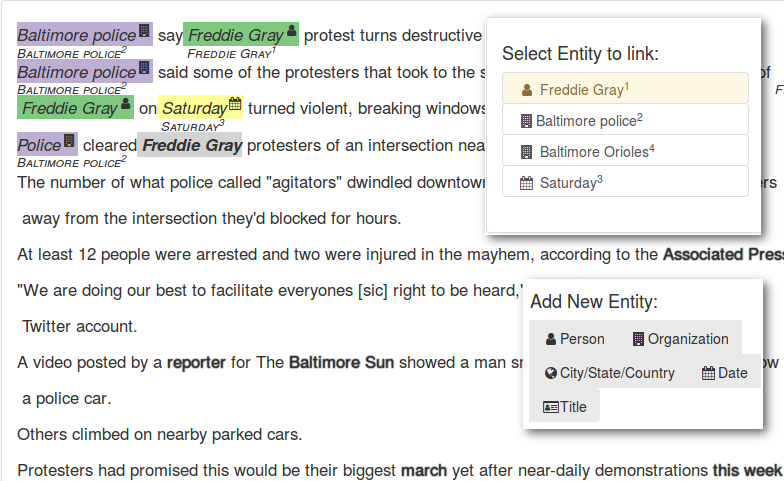
\includegraphics[width=\textwidth]{figures/extraction-interface}
  \caption{\label{fig:extraction-interface} Entity detection and linking.}
\end{subfigure}
\hfill
\begin{subfigure}{0.31\textwidth}
  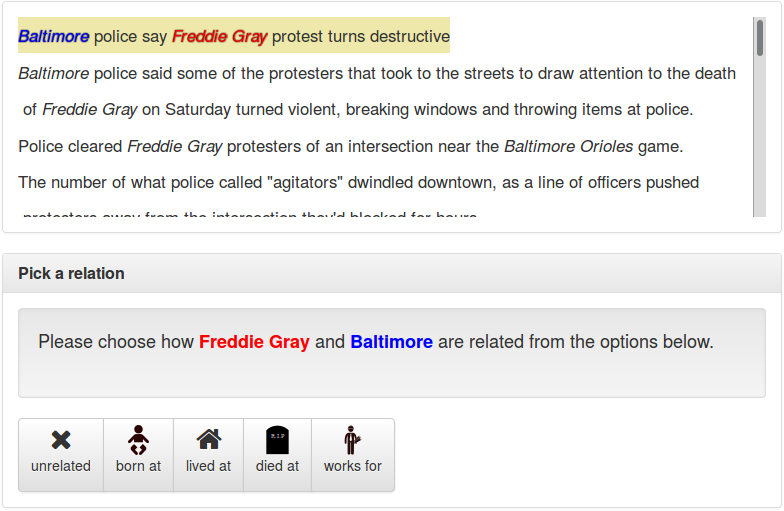
\includegraphics[width=\textwidth]{figures/relation-interface}
  \caption{\label{fig:relation-interface} Relation extraction.}
\end{subfigure}
\hfill
\begin{subfigure}{0.31\textwidth}
  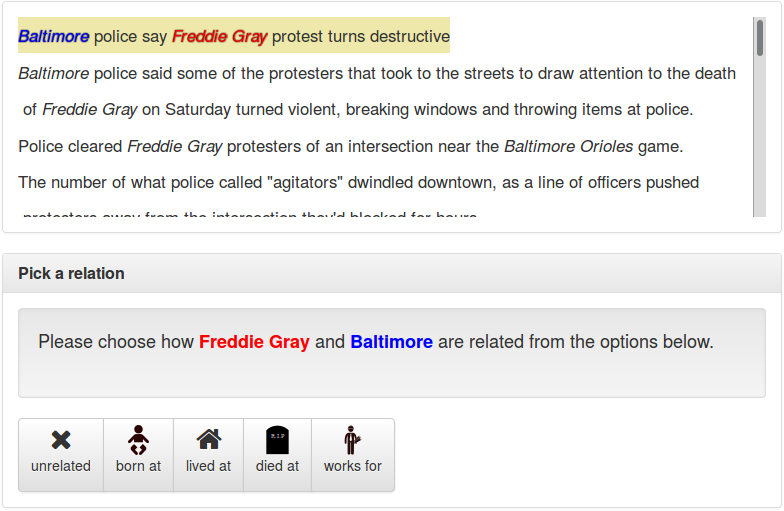
\includegraphics[width=\textwidth]{figures/relation-interface}
  \caption{\label{fig:linking-interface} Cross-document linking.}
\end{subfigure}
% TODO: cross-document linking
%\begin{subfigure}{0.49\textwidth}
%  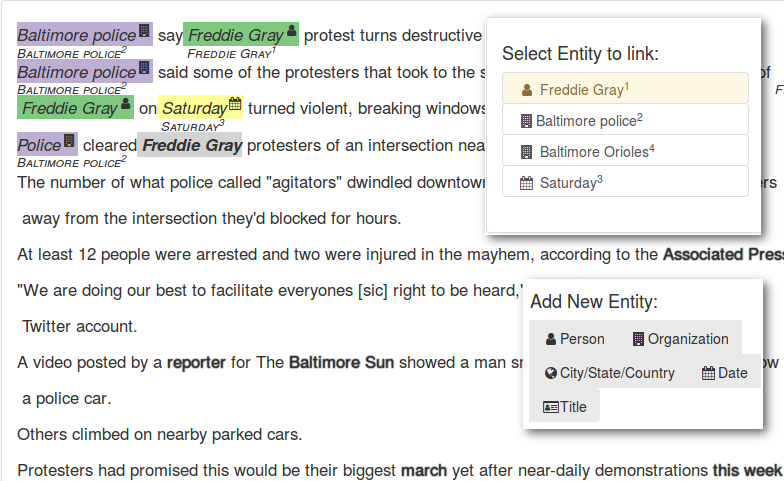
\includegraphics[width=\textwidth]{figures/extraction-interface}
%  \caption{\label{fig:extraction-interface} Exhaustive entity detection and linking.}
%\end{subfigure}
\caption{\label{fig:interfaces} Screenshots of the annotation interfaces.}
\end{figure*}

\paragraph{Exhaustive annotation.}
We can sample documents from the corpus and have crowdworkers exhaustively annotate them.
There are three types of annotations that are required, corresponding to each component of the relation extraction task:
detecting entities in documents, linking them within and across documents and identifying relations between entities in a document. 

% How is the document collection expanded?
When constructing our online evaluation methodology, we must be very careful not to bias the evaluation data we produce towards any particular system. 
There are several modes in which we can obtain annotations on our data.

%\begin{enumerate}
%  \item \textbf{Exhaustive annotation.} 
%    % Include details about the turk interfaces?
%  \item \textbf{Pooling annotation.} 
%    Exhaustively annotating documents is quite laborious and hence expensive to do.
%    Verifying a systems' submission is much easier to do; it takes only \todo{10 seconds} a relation.
%    It also reduces wasted effort in reading text that doesn't contain any relations.
%
%    By including every new submission into the pool, we can avoid the negative consequences of pooling evaluation.
%    Furthermore, we will show how annotations collected in the pooling and exhaustive schemes can be combined to estimate true recall and precision more cheaply.
%
%  \item \textbf{Estimative annotation.} 
%    Finally, we should be able to use agreements between submitting systems as a weak signal of correctness and be able to compute precision and recall on the entire corpus of unannotated contexts.
%    One of the main challenges  we'll have to solve is to make sure that we aren't biasing our scores due to correlations between systems. 
%
%    % TODO: explain using a pooling classifier?
%    % Builds on the previous two systems.
%\end{enumerate}

\paragraph{Combining annotations.}
\ac{Ignore for now!}

Each of the annotation schemes above is advantageous for particular metrics: the exhaustive scheme is necessary for estimating true recall, the pooling scheme is important to reliably estimate precision and the estimative annotation is cheap.

However, we can combine the strengths of these three estimators to allow us to reliably evaluate systems at a fraction of the original cost.

Let us consider how data in the pooling scheme can be used to better estimate recall when combined with the exhaustive annotation.
Let us assume that we have annotated $n_e$ true contexts through the exhaustive annotation, and are able to evaluate the recall of a system $A$ is $r_A$, with some variance $\sigma^2_A$.
We are also able to evaluate the recall of the entire pool $P$ as $r_P$, with variance $\sigma^2_P$.
Let's assume that we can evaluate $n_p$ contexts at random from the pool. 
%The recall of $A$ within the pool is $r'_A$, with variance $\sigma'^2_{A}$.
%We could use the recall of $A$ in the pool to estimate the recall of $A$ as $r_A = r_P * r'_A$.
%The variance of this estimate is $\sigma^2_P \sigma'^2_A + r^2_P \sigma'^2_A + \sigma^2_P r'_A^2$.
%Let's take the limit where estimating pooled recall is very cheap -- in this case, we can take $\sigma'^2_A \to 0$, giving us a new estimate of $r'_A^2 \sigma^2_P$. 
%Noting that recall is a binomial estimator, 
%  we know that $\sigma^2_A = \frac{r_A (1 - r_A)}{n_e}$ and 
%  that $\sigma^2_P = \frac{r_P (1 - r_P)}{n_e}$.
%Thus, our two-step estimator has less variance than the one-step estimator when,
%  $\frac{r'_A^2 r_P (1 - r_P)}{n_e} < \frac{r'_A r_P (1 - r'_A r_P)}{n_e}$, or when $r_'A (1 - r_P) < (1 - r'_A r_P)$.

With a Bernoulli assumption, we get that.

Then, our updated estimate of recall would combine $r_A$ and 

% (2 pages)

\begin{table*}
  \begin{tabular}{l r r r r r r r r} \toprule
    Annotation scheme & Cost per sample & \multicolumn{6}{c}{Information ratio} & Total cost \\ 
                      &                      & $P^m$ & $R^m$ & $F_1^m$ & $P^e$ & $R^e$ & $F_1^e$ &  \\ \midrule
    Exhaustive & \$0.20 & 0.7 & 0.7 & 0.7 & 0.7 & 0.7 & 0.7 & \$1000 \\
    Selective  & \$0.05 & 0.7 & 0.7 & 0.7 & 0.7 & 0.7 & 0.7 & \$1000 \\
    Estimative & \$0.00 & 0.7 & 0.7 & 0.7 & 0.7 & 0.7 & 0.7 &  \\
    Hybrid     & \$0.06 & 0.7 & 0.7 & 0.7 & 0.7 & 0.7 & 0.7 & \$1000 \\ \bottomrule
  \end{tabular}
  \caption{Cost accuracy tradeoffs}
\end{table*}

A motivation for pooling is to reduce cost.
The intuition is in computing recall, we can compute recall against a particular corpus of exhaustively annotated documents,
or compute the recall of the pool with respect to the exhaustive annotations, followed by evaluating the recall of with respect to the pool. 
The latter is much cheaper to evaluate, and as a result, we can get a much more precise annotation on it.
Consider this example to gain intuition as to why incorporating pooling results would help.

Intuition is that if we take two sets of documents and ask for overlap, magic 

